
\documentclass[10pt,twocolumn,letterpaper]{article}
\usepackage[T1]{fontenc}
\usepackage[review]{cvpr}
%% This file contains a number of tweaks that are typically applied to the main document.
%% They are not enabled by default, but can be enabled by uncommenting the relevant lines.

%%
%% Inline annotations; for predefined colors, refer to "dvipsnames" in the xcolor package:
%% https://tinyurl.com/overleaf-colors
%%
\newcommand{\red}[1]{{\color{red}#1}}
\newcommand{\todo}[1]{{\color{red}#1}}
\newcommand{\TODO}[1]{\textbf{\color{red}[TODO: #1]}}
%%
%% disable for camera ready / submission by uncommenting these lines  
%%
% \renewcommand{\TODO}[1]{}
% \renewcommand{\todo}[1]{#1}

%%
%% work harder in optimizing text layout. Typically shrinks text by 1/6 of page, enable
%% it at the very end of the writing process, when you are just above the page limit
%%
% \usepackage{microtype}

%%
%% fine-tune paragraph spacing
%%
% \renewcommand{\paragraph}[1]{\vspace{.5em}\noindent\textbf{#1.}}

%%
%% globally adjusts space between figure and caption
%%
% \setlength{\abovecaptionskip}{.5em}


%%
%% Allows "the use of \paper to refer to the project name"
%% with automatic management of space at the end of the word
%%
% \usepackage{xspace}
% \newcommand{\paper}{ProjectName\xspace}

%%
%% Commonly used math definitions
%%
% \DeclareMathOperator*{\argmin}{arg\,min}
% \DeclareMathOperator*{\argmax}{arg\,max}

%%
%% Tigthen underline
%%
% \usepackage{soul}
% \setuldepth{foobar}
%%%%% NEW MATH DEFINITIONS %%%%%

\usepackage{amsmath,amsfonts,bm}

% Mark sections of captions for referring to divisions of figures
\newcommand{\figleft}{{\em (Left)}}
\newcommand{\figcenter}{{\em (Center)}}
\newcommand{\figright}{{\em (Right)}}
\newcommand{\figtop}{{\em (Top)}}
\newcommand{\figbottom}{{\em (Bottom)}}
\newcommand{\captiona}{{\em (a)}}
\newcommand{\captionb}{{\em (b)}}
\newcommand{\captionc}{{\em (c)}}
\newcommand{\captiond}{{\em (d)}}

% Highlight a newly defined term
\newcommand{\newterm}[1]{{\bf #1}}


% Figure reference, lower-case.
\def\figref#1{figure~\ref{#1}}
% Figure reference, capital. For start of sentence
\def\Figref#1{Figure~\ref{#1}}
\def\twofigref#1#2{figures \ref{#1} and \ref{#2}}
\def\quadfigref#1#2#3#4{figures \ref{#1}, \ref{#2}, \ref{#3} and \ref{#4}}
% Section reference, lower-case.
\def\secref#1{section~\ref{#1}}
% Section reference, capital.
\def\Secref#1{Section~\ref{#1}}
% Reference to two sections.
\def\twosecrefs#1#2{sections \ref{#1} and \ref{#2}}
% Reference to three sections.
\def\secrefs#1#2#3{sections \ref{#1}, \ref{#2} and \ref{#3}}
% Reference to an equation, lower-case.
\def\eqref#1{equation~\ref{#1}}
% Reference to an equation, upper case
\def\Eqref#1{Equation~\ref{#1}}
% A raw reference to an equation---avoid using if possible
\def\plaineqref#1{\ref{#1}}
% Reference to a chapter, lower-case.
\def\chapref#1{chapter~\ref{#1}}
% Reference to an equation, upper case.
\def\Chapref#1{Chapter~\ref{#1}}
% Reference to a range of chapters
\def\rangechapref#1#2{chapters\ref{#1}--\ref{#2}}
% Reference to an algorithm, lower-case.
\def\algref#1{algorithm~\ref{#1}}
% Reference to an algorithm, upper case.
\def\Algref#1{Algorithm~\ref{#1}}
\def\twoalgref#1#2{algorithms \ref{#1} and \ref{#2}}
\def\Twoalgref#1#2{Algorithms \ref{#1} and \ref{#2}}
% Reference to a part, lower case
\def\partref#1{part~\ref{#1}}
% Reference to a part, upper case
\def\Partref#1{Part~\ref{#1}}
\def\twopartref#1#2{parts \ref{#1} and \ref{#2}}

\def\ceil#1{\lceil #1 \rceil}
\def\floor#1{\lfloor #1 \rfloor}
\def\1{\bm{1}}
\newcommand{\train}{\mathcal{D}}
\newcommand{\valid}{\mathcal{D_{\mathrm{valid}}}}
\newcommand{\test}{\mathcal{D_{\mathrm{test}}}}

\def\eps{{\epsilon}}


% Random variables
\def\reta{{\textnormal{$\eta$}}}
\def\ra{{\textnormal{a}}}
\def\rb{{\textnormal{b}}}
\def\rc{{\textnormal{c}}}
\def\rd{{\textnormal{d}}}
\def\re{{\textnormal{e}}}
\def\rf{{\textnormal{f}}}
\def\rg{{\textnormal{g}}}
\def\rh{{\textnormal{h}}}
\def\ri{{\textnormal{i}}}
\def\rj{{\textnormal{j}}}
\def\rk{{\textnormal{k}}}
\def\rl{{\textnormal{l}}}
% rm is already a command, just don't name any random variables m
\def\rn{{\textnormal{n}}}
\def\ro{{\textnormal{o}}}
\def\rp{{\textnormal{p}}}
\def\rq{{\textnormal{q}}}
\def\rr{{\textnormal{r}}}
\def\rs{{\textnormal{s}}}
\def\rt{{\textnormal{t}}}
\def\ru{{\textnormal{u}}}
\def\rv{{\textnormal{v}}}
\def\rw{{\textnormal{w}}}
\def\rx{{\textnormal{x}}}
\def\ry{{\textnormal{y}}}
\def\rz{{\textnormal{z}}}

% Random vectors
\def\rvepsilon{{\mathbf{\epsilon}}}
\def\rvtheta{{\mathbf{\theta}}}
\def\rva{{\mathbf{a}}}
\def\rvb{{\mathbf{b}}}
\def\rvc{{\mathbf{c}}}
\def\rvd{{\mathbf{d}}}
\def\rve{{\mathbf{e}}}
\def\rvf{{\mathbf{f}}}
\def\rvg{{\mathbf{g}}}
\def\rvh{{\mathbf{h}}}
\def\rvu{{\mathbf{i}}}
\def\rvj{{\mathbf{j}}}
\def\rvk{{\mathbf{k}}}
\def\rvl{{\mathbf{l}}}
\def\rvm{{\mathbf{m}}}
\def\rvn{{\mathbf{n}}}
\def\rvo{{\mathbf{o}}}
\def\rvp{{\mathbf{p}}}
\def\rvq{{\mathbf{q}}}
\def\rvr{{\mathbf{r}}}
\def\rvs{{\mathbf{s}}}
\def\rvt{{\mathbf{t}}}
\def\rvu{{\mathbf{u}}}
\def\rvv{{\mathbf{v}}}
\def\rvw{{\mathbf{w}}}
\def\rvx{{\mathbf{x}}}
\def\rvy{{\mathbf{y}}}
\def\rvz{{\mathbf{z}}}

% Elements of random vectors
\def\erva{{\textnormal{a}}}
\def\ervb{{\textnormal{b}}}
\def\ervc{{\textnormal{c}}}
\def\ervd{{\textnormal{d}}}
\def\erve{{\textnormal{e}}}
\def\ervf{{\textnormal{f}}}
\def\ervg{{\textnormal{g}}}
\def\ervh{{\textnormal{h}}}
\def\ervi{{\textnormal{i}}}
\def\ervj{{\textnormal{j}}}
\def\ervk{{\textnormal{k}}}
\def\ervl{{\textnormal{l}}}
\def\ervm{{\textnormal{m}}}
\def\ervn{{\textnormal{n}}}
\def\ervo{{\textnormal{o}}}
\def\ervp{{\textnormal{p}}}
\def\ervq{{\textnormal{q}}}
\def\ervr{{\textnormal{r}}}
\def\ervs{{\textnormal{s}}}
\def\ervt{{\textnormal{t}}}
\def\ervu{{\textnormal{u}}}
\def\ervv{{\textnormal{v}}}
\def\ervw{{\textnormal{w}}}
\def\ervx{{\textnormal{x}}}
\def\ervy{{\textnormal{y}}}
\def\ervz{{\textnormal{z}}}

% Random matrices
\def\rmA{{\mathbf{A}}}
\def\rmB{{\mathbf{B}}}
\def\rmC{{\mathbf{C}}}
\def\rmD{{\mathbf{D}}}
\def\rmE{{\mathbf{E}}}
\def\rmF{{\mathbf{F}}}
\def\rmG{{\mathbf{G}}}
\def\rmH{{\mathbf{H}}}
\def\rmI{{\mathbf{I}}}
\def\rmJ{{\mathbf{J}}}
\def\rmK{{\mathbf{K}}}
\def\rmL{{\mathbf{L}}}
\def\rmM{{\mathbf{M}}}
\def\rmN{{\mathbf{N}}}
\def\rmO{{\mathbf{O}}}
\def\rmP{{\mathbf{P}}}
\def\rmQ{{\mathbf{Q}}}
\def\rmR{{\mathbf{R}}}
\def\rmS{{\mathbf{S}}}
\def\rmT{{\mathbf{T}}}
\def\rmU{{\mathbf{U}}}
\def\rmV{{\mathbf{V}}}
\def\rmW{{\mathbf{W}}}
\def\rmX{{\mathbf{X}}}
\def\rmY{{\mathbf{Y}}}
\def\rmZ{{\mathbf{Z}}}

% Elements of random matrices
\def\ermA{{\textnormal{A}}}
\def\ermB{{\textnormal{B}}}
\def\ermC{{\textnormal{C}}}
\def\ermD{{\textnormal{D}}}
\def\ermE{{\textnormal{E}}}
\def\ermF{{\textnormal{F}}}
\def\ermG{{\textnormal{G}}}
\def\ermH{{\textnormal{H}}}
\def\ermI{{\textnormal{I}}}
\def\ermJ{{\textnormal{J}}}
\def\ermK{{\textnormal{K}}}
\def\ermL{{\textnormal{L}}}
\def\ermM{{\textnormal{M}}}
\def\ermN{{\textnormal{N}}}
\def\ermO{{\textnormal{O}}}
\def\ermP{{\textnormal{P}}}
\def\ermQ{{\textnormal{Q}}}
\def\ermR{{\textnormal{R}}}
\def\ermS{{\textnormal{S}}}
\def\ermT{{\textnormal{T}}}
\def\ermU{{\textnormal{U}}}
\def\ermV{{\textnormal{V}}}
\def\ermW{{\textnormal{W}}}
\def\ermX{{\textnormal{X}}}
\def\ermY{{\textnormal{Y}}}
\def\ermZ{{\textnormal{Z}}}

% Vectors
\def\vzero{{\bm{0}}}
\def\vone{{\bm{1}}}
\def\vmu{{\bm{\mu}}}
\def\vtheta{{\bm{\theta}}}
\def\va{{\bm{a}}}
\def\vb{{\bm{b}}}
\def\vc{{\bm{c}}}
\def\vd{{\bm{d}}}
\def\ve{{\bm{e}}}
\def\vf{{\bm{f}}}
\def\vg{{\bm{g}}}
\def\vh{{\bm{h}}}
\def\vi{{\bm{i}}}
\def\vj{{\bm{j}}}
\def\vk{{\bm{k}}}
\def\vl{{\bm{l}}}
\def\vm{{\bm{m}}}
\def\vn{{\bm{n}}}
\def\vo{{\bm{o}}}
\def\vp{{\bm{p}}}
\def\vq{{\bm{q}}}
\def\vr{{\bm{r}}}
\def\vs{{\bm{s}}}
\def\vt{{\bm{t}}}
\def\vu{{\bm{u}}}
\def\vv{{\bm{v}}}
\def\vw{{\bm{w}}}
\def\vx{{\bm{x}}}
\def\vy{{\bm{y}}}
\def\vz{{\bm{z}}}

% Elements of vectors
\def\evalpha{{\alpha}}
\def\evbeta{{\beta}}
\def\evepsilon{{\epsilon}}
\def\evlambda{{\lambda}}
\def\evomega{{\omega}}
\def\evmu{{\mu}}
\def\evpsi{{\psi}}
\def\evsigma{{\sigma}}
\def\evtheta{{\theta}}
\def\eva{{a}}
\def\evb{{b}}
\def\evc{{c}}
\def\evd{{d}}
\def\eve{{e}}
\def\evf{{f}}
\def\evg{{g}}
\def\evh{{h}}
\def\evi{{i}}
\def\evj{{j}}
\def\evk{{k}}
\def\evl{{l}}
\def\evm{{m}}
\def\evn{{n}}
\def\evo{{o}}
\def\evp{{p}}
\def\evq{{q}}
\def\evr{{r}}
\def\evs{{s}}
\def\evt{{t}}
\def\evu{{u}}
\def\evv{{v}}
\def\evw{{w}}
\def\evx{{x}}
\def\evy{{y}}
\def\evz{{z}}

% Matrix
\def\mA{{\bm{A}}}
\def\mB{{\bm{B}}}
\def\mC{{\bm{C}}}
\def\mD{{\bm{D}}}
\def\mE{{\bm{E}}}
\def\mF{{\bm{F}}}
\def\mG{{\bm{G}}}
\def\mH{{\bm{H}}}
\def\mI{{\bm{I}}}
\def\mJ{{\bm{J}}}
\def\mK{{\bm{K}}}
\def\mL{{\bm{L}}}
\def\mM{{\bm{M}}}
\def\mN{{\bm{N}}}
\def\mO{{\bm{O}}}
\def\mP{{\bm{P}}}
\def\mQ{{\bm{Q}}}
\def\mR{{\bm{R}}}
\def\mS{{\bm{S}}}
\def\mT{{\bm{T}}}
\def\mU{{\bm{U}}}
\def\mV{{\bm{V}}}
\def\mW{{\bm{W}}}
\def\mX{{\bm{X}}}
\def\mY{{\bm{Y}}}
\def\mZ{{\bm{Z}}}
\def\mBeta{{\bm{\beta}}}
\def\mPhi{{\bm{\Phi}}}
\def\mLambda{{\bm{\Lambda}}}
\def\mSigma{{\bm{\Sigma}}}

% Tensor
\DeclareMathAlphabet{\mathsfit}{\encodingdefault}{\sfdefault}{m}{sl}
\SetMathAlphabet{\mathsfit}{bold}{\encodingdefault}{\sfdefault}{bx}{n}
\newcommand{\tens}[1]{\bm{\mathsfit{#1}}}
\def\tA{{\tens{A}}}
\def\tB{{\tens{B}}}
\def\tC{{\tens{C}}}
\def\tD{{\tens{D}}}
\def\tE{{\tens{E}}}
\def\tF{{\tens{F}}}
\def\tG{{\tens{G}}}
\def\tH{{\tens{H}}}
\def\tI{{\tens{I}}}
\def\tJ{{\tens{J}}}
\def\tK{{\tens{K}}}
\def\tL{{\tens{L}}}
\def\tM{{\tens{M}}}
\def\tN{{\tens{N}}}
\def\tO{{\tens{O}}}
\def\tP{{\tens{P}}}
\def\tQ{{\tens{Q}}}
\def\tR{{\tens{R}}}
\def\tS{{\tens{S}}}
\def\tT{{\tens{T}}}
\def\tU{{\tens{U}}}
\def\tV{{\tens{V}}}
\def\tW{{\tens{W}}}
\def\tX{{\tens{X}}}
\def\tY{{\tens{Y}}}
\def\tZ{{\tens{Z}}}


% Graph
\def\gA{{\mathcal{A}}}
\def\gB{{\mathcal{B}}}
\def\gC{{\mathcal{C}}}
\def\gD{{\mathcal{D}}}
\def\gE{{\mathcal{E}}}
\def\gF{{\mathcal{F}}}
\def\gG{{\mathcal{G}}}
\def\gH{{\mathcal{H}}}
\def\gI{{\mathcal{I}}}
\def\gJ{{\mathcal{J}}}
\def\gK{{\mathcal{K}}}
\def\gL{{\mathcal{L}}}
\def\gM{{\mathcal{M}}}
\def\gN{{\mathcal{N}}}
\def\gO{{\mathcal{O}}}
\def\gP{{\mathcal{P}}}
\def\gQ{{\mathcal{Q}}}
\def\gR{{\mathcal{R}}}
\def\gS{{\mathcal{S}}}
\def\gT{{\mathcal{T}}}
\def\gU{{\mathcal{U}}}
\def\gV{{\mathcal{V}}}
\def\gW{{\mathcal{W}}}
\def\gX{{\mathcal{X}}}
\def\gY{{\mathcal{Y}}}
\def\gZ{{\mathcal{Z}}}

% Sets
\def\sA{{\mathbb{A}}}
\def\sB{{\mathbb{B}}}
\def\sC{{\mathbb{C}}}
\def\sD{{\mathbb{D}}}
% Don't use a set called E, because this would be the same as our symbol
% for expectation.
\def\sF{{\mathbb{F}}}
\def\sG{{\mathbb{G}}}
\def\sH{{\mathbb{H}}}
\def\sI{{\mathbb{I}}}
\def\sJ{{\mathbb{J}}}
\def\sK{{\mathbb{K}}}
\def\sL{{\mathbb{L}}}
\def\sM{{\mathbb{M}}}
\def\sN{{\mathbb{N}}}
\def\sO{{\mathbb{O}}}
\def\sP{{\mathbb{P}}}
\def\sQ{{\mathbb{Q}}}
\def\sR{{\mathbb{R}}}
\def\sS{{\mathbb{S}}}
\def\sT{{\mathbb{T}}}
\def\sU{{\mathbb{U}}}
\def\sV{{\mathbb{V}}}
\def\sW{{\mathbb{W}}}
\def\sX{{\mathbb{X}}}
\def\sY{{\mathbb{Y}}}
\def\sZ{{\mathbb{Z}}}

% Entries of a matrix
\def\emLambda{{\Lambda}}
\def\emA{{A}}
\def\emB{{B}}
\def\emC{{C}}
\def\emD{{D}}
\def\emE{{E}}
\def\emF{{F}}
\def\emG{{G}}
\def\emH{{H}}
\def\emI{{I}}
\def\emJ{{J}}
\def\emK{{K}}
\def\emL{{L}}
\def\emM{{M}}
\def\emN{{N}}
\def\emO{{O}}
\def\emP{{P}}
\def\emQ{{Q}}
\def\emR{{R}}
\def\emS{{S}}
\def\emT{{T}}
\def\emU{{U}}
\def\emV{{V}}
\def\emW{{W}}
\def\emX{{X}}
\def\emY{{Y}}
\def\emZ{{Z}}
\def\emSigma{{\Sigma}}

% entries of a tensor
% Same font as tensor, without \bm wrapper
\newcommand{\etens}[1]{\mathsfit{#1}}
\def\etLambda{{\etens{\Lambda}}}
\def\etA{{\etens{A}}}
\def\etB{{\etens{B}}}
\def\etC{{\etens{C}}}
\def\etD{{\etens{D}}}
\def\etE{{\etens{E}}}
\def\etF{{\etens{F}}}
\def\etG{{\etens{G}}}
\def\etH{{\etens{H}}}
\def\etI{{\etens{I}}}
\def\etJ{{\etens{J}}}
\def\etK{{\etens{K}}}
\def\etL{{\etens{L}}}
\def\etM{{\etens{M}}}
\def\etN{{\etens{N}}}
\def\etO{{\etens{O}}}
\def\etP{{\etens{P}}}
\def\etQ{{\etens{Q}}}
\def\etR{{\etens{R}}}
\def\etS{{\etens{S}}}
\def\etT{{\etens{T}}}
\def\etU{{\etens{U}}}
\def\etV{{\etens{V}}}
\def\etW{{\etens{W}}}
\def\etX{{\etens{X}}}
\def\etY{{\etens{Y}}}
\def\etZ{{\etens{Z}}}

% The true underlying data generating distribution
\newcommand{\pdata}{p_{\rm{data}}}
% The empirical distribution defined by the training set
\newcommand{\ptrain}{\hat{p}_{\rm{data}}}
\newcommand{\Ptrain}{\hat{P}_{\rm{data}}}
% The model distribution
\newcommand{\pmodel}{p_{\rm{model}}}
\newcommand{\Pmodel}{P_{\rm{model}}}
\newcommand{\ptildemodel}{\tilde{p}_{\rm{model}}}
% Stochastic autoencoder distributions
\newcommand{\pencode}{p_{\rm{encoder}}}
\newcommand{\pdecode}{p_{\rm{decoder}}}
\newcommand{\precons}{p_{\rm{reconstruct}}}

\newcommand{\laplace}{\mathrm{Laplace}} % Laplace distribution

\newcommand{\E}{\mathbb{E}}
\newcommand{\Ls}{\mathcal{L}}
\newcommand{\R}{\mathbb{R}}
\newcommand{\emp}{\tilde{p}}
\newcommand{\lr}{\alpha}
\newcommand{\reg}{\lambda}
\newcommand{\rect}{\mathrm{rectifier}}
\newcommand{\softmax}{\mathrm{softmax}}
\newcommand{\sigmoid}{\sigma}
\newcommand{\softplus}{\zeta}
\newcommand{\KL}{D_{\mathrm{KL}}}
\newcommand{\Var}{\mathrm{Var}}
\newcommand{\standarderror}{\mathrm{SE}}
\newcommand{\Cov}{\mathrm{Cov}}
% Wolfram Mathworld says $L^2$ is for function spaces and $\ell^2$ is for vectors
% But then they seem to use $L^2$ for vectors throughout the site, and so does
% wikipedia.
\newcommand{\normlzero}{L^0}
\newcommand{\normlone}{L^1}
\newcommand{\normltwo}{L^2}
\newcommand{\normlp}{L^p}
\newcommand{\normmax}{L^\infty}

\newcommand{\parents}{Pa} % See usage in notation.tex. Chosen to match Daphne's book.

\DeclareMathOperator*{\argmax}{arg\,max}
\DeclareMathOperator*{\argmin}{arg\,min}

\DeclareMathOperator{\sign}{sign}
\DeclareMathOperator{\Tr}{Tr}
\let\ab\allowbreak


\definecolor{cvprblue}{rgb}{0.21,0.49,0.74}
\usepackage[pagebackref,breaklinks,colorlinks,allcolors=cvprblue]{hyperref}
\usepackage{amsthm}
\usepackage{float}
\usepackage{array}
\def\paperID{*****}
\def\confName{CVPR}
\def\confYear{2026}
\newcommand{\EditYW}[1]{{\color{red} #1}}
\newcommand{\EditAP}[1]{{\color{blue} #1}}
\newcommand{\EditNL}[1]{{\color{magenta} #1}}
\newcommand{\vect}[1]{\boldsymbol{#1}}
\newtheorem{assumption}{Assumption}
\newtheorem{theorem}{Theorem}

\title{Kinematic Residual Flow Matching for Vision-Language-Action Policies}

\author{Anonymous CVPR 2026 submission}

% The \author macro works with any number of authors. There are two commands
% used to separate the names and addresses of multiple authors: \And and \AND.
%
% Using \And between authors leaves it to \LaTeX{} to determine where to break
% the lines. Using \AND forces a linebreak at that point. So, if \LaTeX{}
% puts 3 of 4 authors names on the first line, and the last on the second
% line, try using \AND instead of \And before the third author name.

\newcommand{\fix}{\marginpar{FIX}}
\newcommand{\new}{\marginpar{NEW}}


% Experiment scaffold: blank numeric cells are deliberately not zero or N/A.
\newcommand{\pending}{\phantom{00.00}}
% Drop a finished PDF at the named path to replace its framed placeholder.
\newcommand{\experimentplot}[4]{%
  \begin{minipage}[c]{#2}\centering
    \IfFileExists{#1}{\includegraphics[width=\linewidth]{#1}}{%
      \fbox{\parbox[c][#3][c]{\dimexpr\linewidth-2\fboxsep-2\fboxrule\relax}{%
        \centering\footnotesize\textbf{Figure pending}\par\smallskip #4}}%
    }%
  \end{minipage}%
}

\begin{document}


\maketitle

\begin{abstract}
Vision-language-action (VLA) policies generate actions from current observations, making them brittle for dynamic manipulation where objects move during execution. We propose \emph{Kinematic-Residual-VLA}, which decomposes action generation into a kinematic branch and a learned residual branch. The kinematic branch projects estimated object velocity into the robot's action space to account for predictable target displacement; a Flow Matching network then learns only the residual manipulation behavior. We call this \emph{Kinematic Residual Flow Matching}. \EditAP{[REWRITE] The key insight is that object velocity is not an arbitrary conditioning variable; it is a physical factor whose first-order effect on actions can be computed analytically and factored out of the learning problem.} \EditAP{[talk about experiments, dataset, backbone and results]}
\end{abstract}


\begin{figure*}[t]
    \centering
    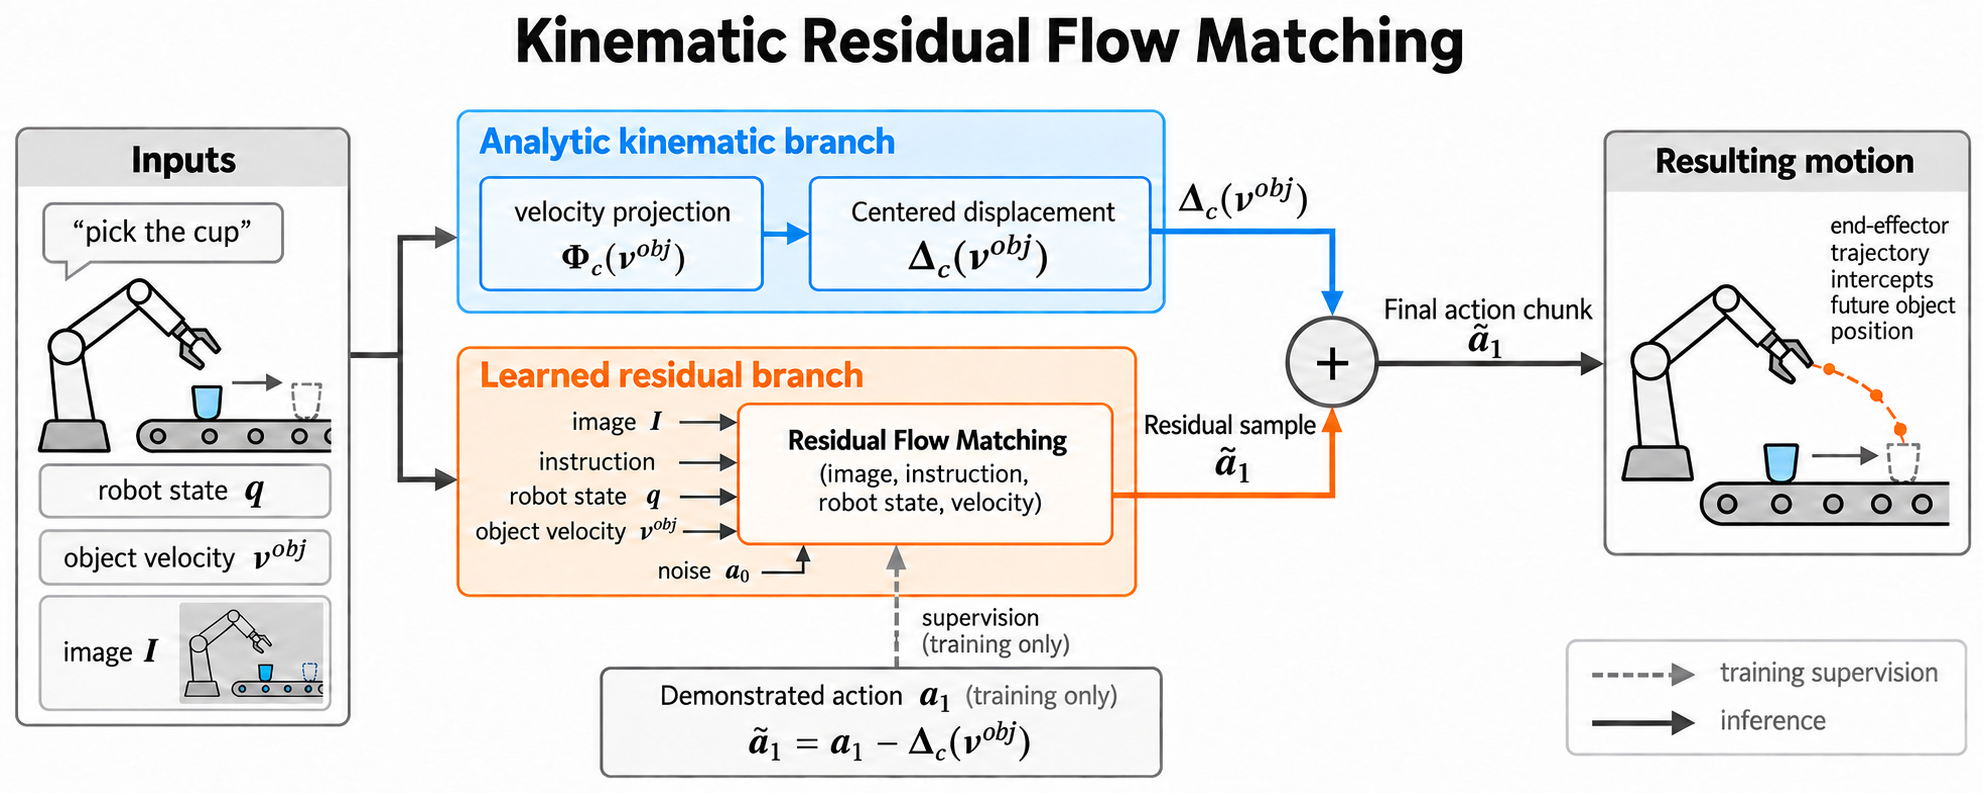
\includegraphics[width=\textwidth]{krfm_overview_v2.png}
    \caption{\textbf{Kinematic Residual Flow Matching.}
    The analytic branch maps object velocity to the centered action displacement
    $\Delta_{\mathbf c}(\mathbf v^{\mathrm{obj}})=d_{\mathbf c}(\mathbf v^{\mathrm{obj}})-\bar d_{\mathbf c}$.
    During training, this displacement is subtracted from the demonstrated
    action chunk to form $\widetilde{\mathbf a}_1$. The learned flow remains
    conditioned on the image, instruction, robot state, and object velocity.
    At inference, a residual sample is combined with the same displacement
    to recover the final action chunk. The illustrated motion is schematic.}
    \label{fig:krfm_overview}
\end{figure*}

\section{Introduction}
\label{sec:intro}

Robots that manipulate moving objects must solve two coupled problems: understanding \emph{what} action is appropriate, and predicting \emph{where the target will be} at contact time. Standard VLA policies address the first problem by conditioning on the current image, language instruction, and robot state \citep{brohan2023rt1,zitkovich2023rt2,kim2024openvla}. This works well in quasi-static scenes, but in tasks such as conveyor-belt picking, catching, or handovers, the observation can already be stale by the time the robot executes the decoded action. Minor latency issues in the VLA can cause task failure, thus making dynamic manipulation even more challenging than static ones.

Current VLA research have attempted to solve the problem of stochasticity in the environment by developing asynchornous inference methods and applying changes to model architecture, that prefer speed over accuracy. A natural response is to provide the policy with predictive information: target velocity, future position estimates, or optical-flow features. However, enriching the input does not simplify the output distribution. We want to seek methods that understand the physical meaning of the object's instrinsics as they try and predict the actions to take so. By simply sending object instrinsics as priviliged input information, we are still not really disentagling its physical meaning within the VLA. 
Majority of the VLA methods out there focus primiarily on static object scenes, or object scenes with simplistic stochasticity. Sometimes, the stochasticity is inherently generated due the VLA's prediction itself, which demands corrective actions by the next action chunk. The solution to most of these methods lies in transforming the model architectures in one way or the other, or finding innovative methods to conduct higher frequency inference.  

A major aspect of our idea is to treat the object instrinsics as a guided residual/disturbance in the flow of the action predicted by the VLA. We want to disenta

The central idea of this paper is to treat object velocity as a \emph{structured nuisance factor} rather than an opaque conditioning token. Over a short action-chunk horizon, object velocity induces a first-order displacement in the desired action that can be projected into the robot's action space via a kinematic map. \emph{Kinematic Residual VLA} removes this projected displacement from the training target, trains a Flow Matching network on the residual $\widetilde{\mathbf a}_1$, and adds the displacement back at inference time. The neural network models residual grasping behavior; the analytic branch handles predictable target motion.

\paragraph{Contributions.}
\begin{itemize}
    \item We introduce \emph{Kinematic Residual Flow Matching} (KRFM), a conditional action-generation method that removes projected velocity displacement from the Flow Matching target and restores it via an analytic drift at inference.
    \item We prove that, under a local additive velocity model, residualization collapses all velocity-conditioned action distributions to a common Wasserstein barycenter and strictly reduces action-target variance (Theorem~\ref{thm:velocity_residualization_reduces_variation}).

\end{itemize}

\section{Related Work}
\label{sec:related}

\paragraph{Vision--language--action policies.}
Large robot policies increasingly use vision-language pretraining and action-token decoding to transfer semantic knowledge into robotic control. RT-1 demonstrated large-scale transformer policies for real-world robot control \citep{brohan2023rt1}. RT-2 framed actions as tokens in a VLA model and showed transfer from web-scale vision-language data to manipulation \citep{zitkovich2023rt2}. OpenVLA provides an open-source VLA trained on broad robot datasets \citep{kim2024openvla}. Kinematic-Residual-VLA is complementary to these systems: it does not require a new backbone, but changes the action expert so that predictable target motion is handled outside the neural residual generator.

\paragraph{Generative action policies.}
Diffusion Policy models visuomotor control as conditional denoising over action sequences \citep{chi2023diffusionpolicy}. Flow Matching trains continuous normalizing flows by regressing vector fields along probability paths \citep{lipman2023flow}. Conditional Flow Matching and minibatch optimal-transport variants connect simulation-free vector-field learning with transport paths between source and target distributions \citep{tong2024improving}. Rectified Flow emphasizes straight transport paths and fast generation \citep{liu2023rectified}. We build on this view by treating action generation as transport from a base action distribution to a demonstration action distribution. The difference is that our target distribution is first expressed in a moving, velocity-disentangled action frame.

\paragraph{Predictive perception for dynamic manipulation.}
The perception interface can be implemented with modern video and geometric modules. Monocular depth estimation provides metric cues \citep{yang2024depthanythingv2}; video segmentation provides target masks \citep{ravi2024sam2}; dense point tracking provides temporal correspondences \citep{karaev2024cotracker}; Lucas--Kanade optical flow and Kalman filtering provide lightweight velocity estimation and uncertainty propagation \citep{lucas1981iterative,kalman1960filtering}. Our theory assumes that such a module produces an estimated target velocity and covariance; it does not depend on a specific tracker.

\paragraph{Optimal transport and variability reduction.}
Wasserstein barycenters define central distributions for probability measures in optimal-transport geometry \citep{agueh2011barycenters,villani2009optimal,peyre2019computational}. Variability reduction with optimal transport uses transport maps to remove nuisance-factor variation by aligning conditional distributions to a common barycenter \citep{hung2022variability}. The dynamic Benamou--Brenier formulation identifies the squared $2$-Wasserstein distance with the minimum kinetic action of a mass-preserving probability flow \citep{benamou2000computational,ambrosio2008gradient}. We specialize these tools to a VLA-specific nuisance factor: target velocity.


\section{Preliminaries: Flow Matching for Action Generation}
\label{sec:prelim}

We model a vision--language--action (VLA) policy as a Conditional Flow
Matching (CFM) generator that predicts an action chunk from an image,
a language instruction, proprioception, and the target object's velocity
\citep{black2025pi0}. \EditAP{[vague sentence. conditioned on what? Combine with next sentence or improve]}
Let $\mathbf c=(\mathcal I,\ell,\mathbf q)$ denote the visual, language,
and robot-state context, and let
$\mathbf c_v=(\mathbf c,\mathbf v^{\mathrm{obj}})$ denote the full policy
conditioning, including the measured object velocity. We keep velocity
explicit so that its effect can be studied at fixed $\mathbf c$. \EditAP{Add the object's velocity as a condition as well}
The output is an $H$-step action sequence
$\mathbf a_{1:H}\in\mathbb R^{H\times d_a}$, where $d_a$ is the per-step
action dimension. We use the same letter for its flattened representation,
$\mathbf a=\operatorname{vec}(\mathbf a_{1:H})\in\mathbb R^d$, with
$d=H d_a$. \EditAP{mention actions as a always. represent the flattended representation as $\mathbf a $ itself}

The conditional data distribution
$p_{\mathrm{data}}(\mathbf a\mid\mathbf c_v)$ describes demonstrated action
chunks associated with the current observations and velocity. During one
generation step, $\mathbf c_v$ and this target distribution are fixed;
they are updated when the robot receives new observations. CFM transports
samples from $p_0=\mathcal N(\mathbf 0,\mathbf I)$ to this distribution
using a learned vector field $\mathbf u_\theta(\mathbf a_s,s,\mathbf c_v)$.
Here $s\in[0,1]$ is a dimensionless \emph{generative flow time}, whereas
$H$ counts future robot execution steps. With control period $\delta t$,
the physical chunk duration is $H\delta t$. Thus, the subscripts $0$, $s$,
and $1$ on flattened chunks refer to flow time, not execution steps.
The schedule $\lambda(s)$ introduced below acts along this generative
coordinate; physical time-to-displacement conversion is part of the
kinematic map. \EditAP{define the conditional action distribution $p_{data}(.|c)$. Does it evolve with time?. Also mention what s means in context here, and how it differs from H (this is important as we have 2 different lambda parameters based on the timings)}

For $\mathbf a_0\sim p_0$,
$\mathbf a_1\sim p_{\mathrm{data}}(\cdot\mid\mathbf c_v)$, and
$s\sim\mathcal U[0,1]$, the interpolation and its target velocity are
\begin{align}
    \mathbf a_s &= (1-s)\mathbf a_0+s\mathbf a_1, \\
    \dot{\mathbf a}_s &= \mathbf a_1-\mathbf a_0.
\end{align}
The CFM objective regresses this endpoint difference:
\begin{equation}
    \mathcal L_{\mathrm{FM}}(\theta)
    = \mathbb E\!\left[
        \left\|\mathbf u_\theta(\mathbf a_s,s,\mathbf c_v)
        -(\mathbf a_1-\mathbf a_0)\right\|_2^2
    \right].
    \label{eq:fm_loss}
\end{equation}
The expectation is over training examples, base samples, and flow time
\citep{lipman2023flow,tong2023conditional}. At inference, we sample
$\mathbf a_0\sim p_0$ and integrate
$d\mathbf a_s/ds=\mathbf u_\theta(\mathbf a_s,s,\mathbf c_v)$ from
$s=0$ to $s=1$. The generated endpoint is reshaped into an action
sequence for robot execution.

\section{Kinematic Residual Flow Matching}
\label{sec:method}

Figure~\ref{fig:krfm_overview} summarizes our proposed approach. Section~\ref{subsec:problem_setting} defines the
dynamic manipulation setting and our core modeling assumption.
Sections~\ref{subsec:kinematic_projection}--\ref{subsec:residual_target}
introduce the kinematic velocity projection and the residual training target.
Section~\ref{subsec:variance_reduction} gives the variance-reduction analysis,
and Section~\ref{subsec:inference} describes inference.

\subsection{Problem Setting}
\label{subsec:problem_setting}

We consider manipulation of objects that move during action execution.
Each training example contains the current context, object velocity,
and an expert action chunk:
\[
    \mathcal D=\left\{
    (\mathbf c^{(i)},\mathbf v^{\mathrm{obj},(i)},\mathbf a_1^{(i)})
    \right\}_{i=1}^N.
\]
Here $\mathbf a_1^{(i)}$ is the flattened demonstrated sequence: the desired
output that supervises the policy for example $i$. \EditAP{[what is supervised target]}
Its conditional distribution is
$p_{\mathrm{data}}(\cdot\mid\mathbf c,\mathbf v^{\mathrm{obj}})$.

A velocity-conditioned CFM policy learns to generate these raw actions.
Even for the same scene and manipulation objective, a faster target may
require a larger displacement of the end effector before contact.
Consequently, changing target velocity shifts the required action chunks,
and the model must learn these shifts along with the remaining task
behavior. This adds variation \emph{across} velocity-conditioned targets;
it does not imply that each fixed-velocity distribution has larger variance.
\EditAP{explain this paragraph better. What does the last line mean?}
We use the observed velocity both as a policy input and to compute an
explicit action-space correction, so that the network learns from targets
with the predictable displacement removed.

\paragraph{Residual distribution and local modeling assumption.}
Let $d_{\mathbf c}(\mathbf v^{\mathrm{obj}})\in\mathbb R^d$ denote the
kinematically predicted displacement over the action chunk, defined in
Section~\ref{subsec:kinematic_projection}. For a demonstrated chunk
$\mathbf a_1$, define the uncentered residual
$\mathbf r=\mathbf a_1-d_{\mathbf c}(\mathbf v^{\mathrm{obj}})$.
The distribution of these transformed demonstrations at fixed context and
velocity is $p_{\mathrm{res}}(\cdot\mid\mathbf c,\mathbf v^{\mathrm{obj}})$.
Writing $\tau_{\mathbf b}$ for translation by $\mathbf b$ gives
\begin{align}
    &\tau_{\mathbf b}(\mathbf a)=\mathbf a+\mathbf b, \notag\\
    &p_{\mathrm{data}}(\cdot\mid\mathbf c_v) \notag\\
    &\qquad=\bigl(\tau_{d_{\mathbf c}(\mathbf v^{\mathrm{obj}})}\bigr)_{\#}
    p_{\mathrm{res}}(\cdot\mid\mathbf c_v).
    \label{eq:residual_pushforward_identity}
\end{align}
The pushforward symbol $\#$ means applying the map to every sample of a
distribution. Physically, this translation adds the predicted motion
compensation to a residual action chunk to recover the original action.
The equality follows from the residual definition and does not assume
that the residual is independent of velocity.

Our \emph{local additive model} makes the additional approximation that,
over a short chunk with nearly constant target velocity and locally valid
kinematics, this translation accounts for the dominant velocity dependence:
\begin{align}
    &p_{\mathrm{res}}(\cdot\mid\mathbf c_v)
    \approx p_{\mathrm{res}}(\cdot\mid\mathbf c), \notag\\
    &p_{\mathrm{data}}(\cdot\mid\mathbf c_v) \notag\\
    &\qquad\approx\bigl(\tau_{d_{\mathbf c}(\mathbf v^{\mathrm{obj}})}\bigr)_{\#}
    p_{\mathrm{res}}(\cdot\mid\mathbf c).
    \label{eq:velocity_pushforward_model}
\end{align}
\EditAP{use align for above equations}
The residual represents the action component left after this correction;
we do not impose a particular number or type of grasp modes. \EditAP{definition of multi-modal is different. For this paper, we are not delving on the different types of grasp modes, so we do not need to focus on that aspect as lot.}
In practice, the residual generator remains conditioned on
$\mathbf c_v=(\mathbf c,\mathbf v^{\mathrm{obj}})$ and can learn
velocity-dependent effects that the local projection does not capture.
The exact conditional-independence assumption used for the variance and
optimal-transport guarantees is stated separately in
Assumption~\ref{ass:local_residual_kinematic_model}. Residualization alone
does not guarantee that assumption. Section~\ref{subsec:residual_target}
adds an optional centering term to obtain the training target
$\widetilde{\mathbf a}_1$.
\EditAP{the above paragraph needs quite some refinement. Reform it to be technically sharper. What is the assumption we are making here? What does $\tau$ and $\#$ mean here. What is the physcial meaning of the pushforward operator on the residual action distribution. I don't think we have even defined what the residual action distribution is before this. Another important factor is that even though we calculate the residual action distribution during training, it is still conditioned on the object velocity (which makes it easier for us to make the grasps mode independent and data dependent rather).}

\subsection{Kinematic Velocity Projection}
\label{subsec:kinematic_projection}

The object velocity $\mathbf v^{\mathrm{obj}}$ is expressed in the robot base
frame, whereas the target $\mathbf a_1$ is a flattened action chunk.
We define $\Phi_{\mathbf c}:\mathbb R^{d_{\mathrm{obj}}}\rightarrow\mathbb R^d$
to express motion compensation in the policy's action coordinates;
$d_{\mathrm{obj}}=3$ for translational object velocity.
The map depends on the action representation and the physical times
associated with the chunk entries.

For joint-space actions, a local kinematic map is
\begin{equation}
    \Phi_{\mathbf c}(\mathbf v^{\mathrm{obj}})
    =L_H J^\dagger(\mathbf q)R_{\mathbf c}\mathbf v^{\mathrm{obj}}.
    \label{eq:kinematic_projection}
\end{equation}
Here $R_{\mathbf c}$ rotates velocity into the Jacobian's reference frame,
$J^\dagger(\mathbf q)$ maps Cartesian velocity to joint velocity, and $L_H$
converts and stacks it into the $H$ action entries
\citep{nakamura1991advanced,siciliano2009robotics}.
To compute these terms, use the calibrated frame transform for
$R_{\mathbf c}$ (the identity when both quantities use the base frame),
evaluate the translational Jacobian from the robot kinematic model at the
measured joint configuration $\mathbf q$, and obtain its pseudoinverse by
singular-value decomposition.
Construct $L_H$ from the action timestamps: for position targets or offsets
relative to the current configuration, its $k$th block scales joint velocity
by the look-ahead time $T_k$; for successive position increments it scales by
the interval $\delta t_k$, and for velocity commands it uses unit scaling.
\EditAP{[also mention how we would ideally calculate each term here in one-two sentences]}
For Cartesian position actions, the Jacobian inverse is unnecessary:
the corresponding correction is $T_k R_{\mathbf c}\mathbf v^{\mathrm{obj}}$.
The translational correction has zero entries in orientation, gripper, and
padding channels. The projection is local to a short chunk; it does not
model full-episode dynamics or contact constraints.

We express the integrated displacement as
\begin{align}
    d_{\mathbf c}(\mathbf v^{\mathrm{obj}})
    &=\Lambda\Phi_{\mathbf c}(\mathbf v^{\mathrm{obj}}), \\
    \Lambda&=\int_0^1\lambda(s)\,ds.
    \label{eq:integrated_velocity_displacement}
\end{align}
Physical time factors belong to $L_H$; $\lambda(s)$ is a schedule over
generative flow time. Choosing $\lambda(s)=1$ gives $\Lambda=1$, avoiding a
second multiplication by the physical horizon.
If actions are normalized by an affine map $N(\mathbf a)=S\mathbf a+\mathbf b$,
the physical correction is mapped by $S$ alone, so subtraction and addition
use the same units as the training targets.

These choices reflect existing VLA interfaces: OpenVLA discretizes normalized
end-effector deltas and gripper commands~\citep{kim2024openvla}; DynamicVLA
predicts end-effector pose and gripper-state chunks~\citep{xie2026dynamicvla};
and $\pi_0$ generates continuous action chunks across robot
embodiments~\citep{black2025pi0}. KRFM operates on continuous action
coordinates; discrete token indices are not an additive action space.
\EditAP{why these action chunk values, because thats what x,y,z VLA's predict. Cite those VLA's here.}

\subsection{Residual Training Target}
\label{subsec:residual_target}

For a fixed context $\mathbf c$, let $\mathbf v^{\mathrm{obj}}$ denote the random object
velocity in the dataset. We center the kinematic displacement as
\[
    \bar d_{\mathbf c}
    =
    \mathbb E[d_{\mathbf c}(\mathbf v^{\mathrm{obj}})\mid\mathbf c],
    \qquad
    \Delta_{\mathbf c}(\mathbf v^{\mathrm{obj}})
    =
    d_{\mathbf c}(\mathbf v^{\mathrm{obj}})-\bar d_{\mathbf c}.
\]
The residual training target is then
\begin{equation}
    \widetilde{\mathbf a}_1
    =
    \mathbf a_1-\Delta_{\mathbf c}(\mathbf v^{\mathrm{obj}})
    =
    \mathbf a_1-d_{\mathbf c}(\mathbf v^{\mathrm{obj}})+\bar d_{\mathbf c}.
    \label{eq:residual_target}
\end{equation}
The centering term $\bar d_{\mathbf c}$ is not required to construct a valid
residual target: in practice, one may simply train on
$\mathbf a_1-d_{\mathbf c}(\mathbf v^{\mathrm{obj}})$, which already removes the
velocity-dependent displacement from the supervision signal. Its role is instead
statistical. If the average kinematic displacement is nonzero under context
$\mathbf c$, subtracting $d_{\mathbf c}(\mathbf v^{\mathrm{obj}})$ alone shifts the
conditional mean of the target distribution:
\[
    \mathbb E[\mathbf a_1-d_{\mathbf c}(\mathbf V^{\mathrm{obj}})\mid \mathbf c]
    =
    \mathbb E[\mathbf a_1\mid \mathbf c]
    -
    \mathbb E[d_{\mathbf c}(\mathbf V^{\mathrm{obj}})\mid \mathbf c].
\]
Adding back $\bar d_{\mathbf c}$ makes the residualization mean-preserving,
since
\[
    \mathbb E[\widetilde{\mathbf a}_1\mid \mathbf c]
    =
    \mathbb E[\mathbf a_1\mid \mathbf c].
\]
Thus, centering removes the velocity-induced fluctuation
$d_{\mathbf c}(\mathbf V^{\mathrm{obj}})-\bar d_{\mathbf c}$ while keeping the residual
target at the same conditional barycenter as the original action distribution.
This is desirable statistically because the learned flow models a lower-variance
residual distribution without being forced to compensate for an artificial mean
shift. When the velocity-induced displacement is already centered within a task,
or when estimating $\bar d_{\mathbf c}$ is inconvenient, setting
$\bar d_{\mathbf c}=0$ remains a valid and simple implementation choice.

The residual Flow Matching path uses the same base sample $\mathbf a_0\sim p_0$
as the standard VLA objective, but it connects $\mathbf a_0$ to
$\widetilde{\mathbf a}_1$ rather than to the raw target $\mathbf a_1$:
\[
    \widetilde{\mathbf a}_s
    =
    (1-s)\mathbf a_0+s\widetilde{\mathbf a}_1,
    \qquad
    s\sim\mathcal U[0,1].
\]
The Kinematic Residual Flow Matching loss is
\begin{equation}
    \mathcal L_{\mathrm{KRFM}}(\theta)
    =
    \mathbb E
    \left[
        \left\|
            \mathbf u_\theta(\widetilde{\mathbf a}_s,s,\mathbf c_v)
            -
            (\widetilde{\mathbf a}_1-\mathbf a_0)
        \right\|_2^2
    \right].
    \label{eq:krfm_loss}
\end{equation}
Compared with direct Flow Matching on $\mathbf a_1$, this objective changes the
target distribution rather than merely adding another conditioning variable. The
network remains conditioned on $\mathbf c_v$ and is trained to model the residual action distribution, while the
kinematic branch accounts for the predictable object-motion displacement.

\subsection{Inference}
\label{subsec:inference}

For each observation, we hold $\mathbf c_v$ and its projected displacement
fixed during one flow solve. Starting from $\mathbf a_0\sim p_0$, the
residual generator integrates
\begin{align}
    \frac{d\widetilde{\mathbf a}_s}{ds}
    &=\mathbf u_\theta(\widetilde{\mathbf a}_s,s,\mathbf c_v), \\
    \widetilde{\mathbf a}_0&=\mathbf a_0,
\end{align}
producing $\widehat{\widetilde{\mathbf a}}_1$. We then invert the target
transformation in Eq.~\ref{eq:residual_target}:
\begin{align}
    \widehat{\mathbf a}_1
    &=\widehat{\widetilde{\mathbf a}}_1
      +\Delta_{\mathbf c}(\mathbf v^{\mathrm{obj}}) \notag\\
    &=\widehat{\widetilde{\mathbf a}}_1
      +d_{\mathbf c}(\mathbf v^{\mathrm{obj}})-\bar d_{\mathbf c}.
    \label{eq:residual_to_raw_inference}
\end{align}
The added term is an action-space displacement with the appropriate frame,
horizon, and normalization, rather than the raw object velocity.
The network was trained on actions with this same term removed; adding it
back restores the original action coordinates. Applying an extra displacement
to a policy trained on raw actions would be a different procedure and could
count learned motion compensation twice.

This reconstruction also has an equivalent flow formulation.
Writing $\Delta=\Delta_{\mathbf c}(\mathbf v^{\mathrm{obj}})$ for the fixed
chunk displacement, define a translated path:
\begin{align}
    \mathbf a_s&=\widetilde{\mathbf a}_s+s\Delta, \\
    \frac{d\mathbf a_s}{ds}
    &=\mathbf u_\theta(\mathbf a_s-s\Delta,s,\mathbf c_v)+\Delta.
    \label{eq:translated_action_flow}
\end{align}
The second line follows by differentiation. Thus, endpoint reconstruction
and integrating this analytically shifted flow yield the same endpoint
in continuous time. The shifted network input is essential to this equivalence.
The additive reconstruction is deliberately simple; the modeling change is
the coordinated transformation of training targets and generated samples.
Any benefit depends on the accuracy of the local kinematic model and must be
established by the matched ablations in Section~\ref{sec:experiments}.

Finally, we undo action normalization, reshape the generated chunk, and execute
it through the existing controller. At the next observation, context and
velocity are updated and the process repeats in a receding horizon.
\EditAP{Do we simply add the object velocity conditioned residual to the final action chunk? Isn't this a little rudimentary}

\subsection{Variance Reduction Analysis}
\label{subsec:variance_reduction}

We now formalize the variance-reduction effect of kinematic residualization.
The analysis is local: it is not intended as a global model of manipulation
dynamics, but rather as a short-horizon approximation over one action chunk. In
this regime, constant-velocity prediction and local kinematic projection provide
a first-order description of how object motion shifts the expert action target.

\begin{assumption}[Local residual-plus-kinematic action model]
\label{ass:local_residual_kinematic_model}
Fix a context value $\mathbf c$ (excluding object velocity). We use uppercase
$\mathbf A_1$ for the random action chunk whose samples are $\mathbf a_1$.
The raw expert action target admits the
decomposition
\begin{equation}
    \mathbf A_1
    =
    \mathbf R_{\mathbf c}
    +
    d_{\mathbf c}(\mathbf v^{\mathrm{obj}}),
    \label{eq:local_residual_kinematic_model}
\end{equation}
where $\mathbf R_{\mathbf c}$ is a residual action random variable,
$d_{\mathbf c}(\mathbf v^{\mathrm{obj}})$ is the projected object-velocity displacement in
the action space, both terms have finite second moments, and
\[
    \mathbf R_{\mathbf c}
    \perp\!\!\!\perp
    \mathbf v^{\mathrm{obj}}
    \mid
    \mathbf c.
\]
\end{assumption}

Assumption~\ref{ass:local_residual_kinematic_model} states that, conditioned on
the context, the raw action target consists of two components: a residual
manipulation component and a predictable kinematic displacement induced by
object velocity. The residual component may still be complex and multimodal; it
may encode different grasps, contact strategies, approach directions, or other
task-dependent choices. The assumption only requires that object velocity acts
locally as an additive shift of the action chunk after projection through
$d_{\mathbf c}(\cdot)$. Thus, the same residual manipulation modes should not
need to be relearned as separate action modes for every observed object
velocity.

For a generic action target $\mathbf Y$, let
\[
    \eta_{\mathbf v^{\mathrm{obj}}}^{\mathbf Y}
    :=
    \mathcal L(\mathbf Y \mid \mathbf v^{\mathrm{obj}}=\mathbf v^{\mathrm{obj}},\mathbf c)
\]
denote its velocity-conditioned law. Following Wasserstein barycenters and
optimal-transport variability reduction
\citep{agueh2011barycenters,villani2009optimal,hung2022variability}, define the
velocity-induced OT variability of $\mathbf Y$ as
\begin{equation}
    \mathcal V_{\mathrm{OT}}(\mathbf Y;\mathbf v^{\mathrm{obj}}\mid\mathbf c)
    :=
    \inf_{\nu\in\mathcal P_2(\mathbb R^d)}
    \mathbb E
    \left[
        W_2^2
        \left(
            \eta_{\mathbf v^{\mathrm{obj}}}^{\mathbf Y},
            \nu
        \right)
        \mid \mathbf c
    \right].
    \label{eq:velocity_ot_variability}
\end{equation}
This quantity measures how far the conditional action distribution moves as the
object velocity changes.

\begin{theorem}[Object-velocity residualization reduces target variation]
\label{thm:velocity_residualization_reduces_variation}
Under Assumption~\ref{ass:local_residual_kinematic_model}, define the
residualized target
\begin{equation}
    \widetilde{\mathbf A}_1
    =
    \mathbf A_1
    -
    d_{\mathbf c}(\mathbf v^{\mathrm{obj}})
    +
    \bar d_{\mathbf c},
    \qquad
    \bar d_{\mathbf c}
    =
    \mathbb E
    [
        d_{\mathbf c}(\mathbf v^{\mathrm{obj}})
        \mid
        \mathbf c
    ].
    \label{eq:residualized_target_variance_analysis}
\end{equation}
Then all velocity-conditioned residual target laws are identical:
\begin{equation}
    \mathcal L
    \left(
        \widetilde{\mathbf A}_1
        \mid
        \mathbf v^{\mathrm{obj}}=\mathbf v^{\mathrm{obj}},
        \mathbf c
    \right)
    =
    \mathcal L
    \left(
        \mathbf R_{\mathbf c}
        +
        \bar d_{\mathbf c}
        \mid
        \mathbf c
    \right)
    \quad
    \text{for all } \mathbf v^{\mathrm{obj}}.
    \label{eq:residual_laws_identical}
\end{equation}
Consequently,
\begin{equation}
    \mathcal V_{\mathrm{OT}}
    (
        \widetilde{\mathbf A}_1;
        \mathbf v^{\mathrm{obj}}
        \mid
        \mathbf c
    )
    =
    0.
    \label{eq:residual_ot_zero}
\end{equation}
In contrast, the raw target satisfies
\begin{equation}
    \mathcal V_{\mathrm{OT}}
    (
        \mathbf A_1;
        \mathbf v^{\mathrm{obj}}
        \mid
        \mathbf c
    )
    =
    \mathbb E
    \left[
        \left\|
            d_{\mathbf c}(\mathbf v^{\mathrm{obj}})
            -
            \bar d_{\mathbf c}
        \right\|_2^2
        \mid
        \mathbf c
    \right].
    \label{eq:ot_variability_value}
\end{equation}
Moreover, the residualized target covariance satisfies
\begin{equation}
    \operatorname{tr}
    \operatorname{Cov}
    (
        \widetilde{\mathbf A}_1
        \mid
        \mathbf c
    )
    =
    \operatorname{tr}
    \operatorname{Cov}
    (
        \mathbf A_1
        \mid
        \mathbf c
    )
    -
    \operatorname{tr}
    \operatorname{Cov}
    (
        d_{\mathbf c}(\mathbf v^{\mathrm{obj}})
        \mid
        \mathbf c
    ).
    \label{eq:covariance_reduction}
\end{equation}
Thus, whenever the projected object-velocity displacement has nonzero
conditional covariance, the residualized target has strictly smaller total
variance than the raw action target.
\end{theorem}

\paragraph{Interpretation.}
The baseline VLA is trained on raw expert actions $\mathbf A_1$, whose
variation reflects both residual manipulation choices and object-motion
compensation. Under Assumption~\ref{ass:local_residual_kinematic_model}, object
velocity creates translated copies of the same residual action distribution.
Kinematic residualization subtracts the velocity-specific displacement
$d_{\mathbf c}(\mathbf v^{\mathrm{obj}})$ and adds back its conditional mean
$\bar d_{\mathbf c}$, thereby aligning these translated distributions at a
common center. The residualized target therefore removes variation that is
explained by first-order object motion, while preserving the residual
manipulation distribution that the policy must still learn. For a Flow Matching
VLA, this means that the terminal action distribution used for training has less
velocity-induced spread; the learned generative velocity field no longer needs
to model repeated, velocity-shifted copies of the same manipulation modes.

\begin{proof}
Let
\[
    \mathbf D_{\mathbf c}
    :=
    d_{\mathbf c}(\mathbf v^{\mathrm{obj}}).
\]
By Assumption~\ref{ass:local_residual_kinematic_model},
\[
    \mathbf A_1
    =
    \mathbf R_{\mathbf c}
    +
    \mathbf D_{\mathbf c}.
\]
Substituting this expression into
Eq.~\eqref{eq:residualized_target_variance_analysis} gives
\[
    \widetilde{\mathbf A}_1
    =
    \mathbf R_{\mathbf c}
    +
    \mathbf D_{\mathbf c}
    -
    \mathbf D_{\mathbf c}
    +
    \bar d_{\mathbf c}
    =
    \mathbf R_{\mathbf c}
    +
    \bar d_{\mathbf c}.
\]
Since
$\mathbf R_{\mathbf c}\perp\!\!\!\perp \mathbf v^{\mathrm{obj}}\mid\mathbf c$, the
conditional law of $\mathbf R_{\mathbf c}$ does not depend on the realized
velocity value $\mathbf v^{\mathrm{obj}}$. Hence, for every $\mathbf v^{\mathrm{obj}}$,
\[
    \mathcal L
    \left(
        \widetilde{\mathbf A}_1
        \mid
        \mathbf v^{\mathrm{obj}}=\mathbf v^{\mathrm{obj}},
        \mathbf c
    \right)
    =
    \mathcal L
    \left(
        \mathbf R_{\mathbf c}
        +
        \bar d_{\mathbf c}
        \mid
        \mathbf c
    \right),
\]
which proves Eq.~\eqref{eq:residual_laws_identical}. Since all
velocity-conditioned residual laws are identical, choosing this common law as
the barycenter in Eq.~\eqref{eq:velocity_ot_variability} yields
Eq.~\eqref{eq:residual_ot_zero}.

It remains to compute the OT variability of the raw target. Let
\[
    \rho_{\mathbf c}
    :=
    \mathcal L(\mathbf R_{\mathbf c}\mid\mathbf c).
\]
For each velocity value $\mathbf v^{\mathrm{obj}}$, the raw conditional law is
\[
    \mathcal L
    (
        \mathbf A_1
        \mid
        \mathbf v^{\mathrm{obj}}=\mathbf v^{\mathrm{obj}},
        \mathbf c
    )
    =
    (T_{d_{\mathbf c}(\mathbf v^{\mathrm{obj}})})_{\#}\rho_{\mathbf c},
\]
where $T_{\mathbf a}(\mathbf z)=\mathbf z+\mathbf a$ denotes translation by
$\mathbf a$. Thus, the raw velocity-conditioned laws are translations of the
same residual law. Taking
\[
    \nu^\star
    =
    (T_{\bar d_{\mathbf c}})_{\#}\rho_{\mathbf c}
\]
gives the upper bound
\[
    W_2^2
    \left(
        (T_{d_{\mathbf c}(\mathbf v^{\mathrm{obj}})})_{\#}\rho_{\mathbf c},
        (T_{\bar d_{\mathbf c}})_{\#}\rho_{\mathbf c}
    \right)
    \le
    \left\|
        d_{\mathbf c}(\mathbf v^{\mathrm{obj}})
        -
        \bar d_{\mathbf c}
    \right\|_2^2.
\]
This bound is tight because the optimal coupling between two translated copies
of the same distribution is obtained by applying the corresponding translation.
Therefore,
\[
    \mathcal V_{\mathrm{OT}}
    (
        \mathbf A_1;
        \mathbf v^{\mathrm{obj}}
        \mid
        \mathbf c
    )
    \le
    \mathbb E
    \left[
        \left\|
            d_{\mathbf c}(\mathbf v^{\mathrm{obj}})
            -
            \bar d_{\mathbf c}
        \right\|_2^2
        \mid
        \mathbf c
    \right].
\]
Conversely, for any $\nu\in\mathcal P_2(\mathbb R^d)$ with mean
$m_{\nu}$, the Wasserstein distance lower bounds the squared distance between
means:
\[
    W_2^2
    \left(
        (T_{d_{\mathbf c}(\mathbf v^{\mathrm{obj}})})_{\#}\rho_{\mathbf c},
        \nu
    \right)
    \ge
    \left\|
        m_{\rho_{\mathbf c}}
        +
        d_{\mathbf c}(\mathbf v^{\mathrm{obj}})
        -
        m_{\nu}
    \right\|_2^2,
\]
where $m_{\rho_{\mathbf c}}$ is the mean of $\rho_{\mathbf c}$. Minimizing the
right-hand side over $m_{\nu}$ yields
$m_{\nu}=m_{\rho_{\mathbf c}}+\bar d_{\mathbf c}$ and gives the lower bound
\[
    \mathbb E
    \left[
        \left\|
            d_{\mathbf c}(\mathbf v^{\mathrm{obj}})
            -
            \bar d_{\mathbf c}
        \right\|_2^2
        \mid
        \mathbf c
    \right].
\]
The matching upper and lower bounds prove
Eq.~\eqref{eq:ot_variability_value}.

Finally, using the additive decomposition and conditional independence,
\[
    \operatorname{Cov}
    (
        \mathbf A_1
        \mid
        \mathbf c
    )
    =
    \operatorname{Cov}
    (
        \mathbf R_{\mathbf c}
        \mid
        \mathbf c
    )
    +
    \operatorname{Cov}
    (
        d_{\mathbf c}(\mathbf v^{\mathrm{obj}})
        \mid
        \mathbf c
    ).
\]
On the other hand,
\[
    \widetilde{\mathbf A}_1
    =
    \mathbf R_{\mathbf c}
    +
    \bar d_{\mathbf c},
\]
and $\bar d_{\mathbf c}$ is constant conditioned on $\mathbf c$, so
\[
    \operatorname{Cov}
    (
        \widetilde{\mathbf A}_1
        \mid
        \mathbf c
    )
    =
    \operatorname{Cov}
    (
        \mathbf R_{\mathbf c}
        \mid
        \mathbf c
    ).
\]
Subtracting these two identities and taking traces gives
Eq.~\eqref{eq:covariance_reduction}. Since covariance matrices are positive
semidefinite, a nonzero
$\operatorname{Cov}(d_{\mathbf c}(\mathbf v^{\mathrm{obj}})\mid\mathbf c)$ has positive
trace, yielding strict reduction in total variance.
\end{proof}


\section{Experiments}
\label{sec:experiments}

We study Kinematic Residual Flow Matching (KRFM) within the DynamicVLA
framework~\citep{xie2026dynamicvla}. The experiments address three questions:
does residualizing the action target improve dynamic manipulation; does it
help under changes in object motion; and can any benefit be attributed to the
kinematic decomposition rather than additional velocity information or training?
We distinguish the released DynamicVLA checkpoint from matched fine-tuned
DynamicVLA variants throughout.
\TODO{Draft status: only the locally evaluated released DynamicVLA row is
complete. Empty result cells and framed figures await measurements; proposed
analyses below are not claims of completed experiments.}

\subsection{Experimental Setup}
\label{sec:exp_setup}

\paragraph{Benchmark and protocol.}
Our primary evaluation uses the released Dynamic Object Manipulation (DOM)
simulation suite~\citep{xie2026dynamicvla}. Table~\ref{tab:dom_main} follows
Table~1 of the cited paper (arXiv v2), grouping nine dimensions into interaction,
perception, and generalization. The suite contains 90 released configurations,
with ten configurations per dimension and 20 trials per configuration, for
1,800 trials per complete evaluation. We preserve the configuration files,
reset seeds, task termination rules, and continuous inference with
latency-aware action streaming. Success means completing the instructed
manipulation; proximity to the moving object alone does not count as success.

The completed released-checkpoint evaluation uses Isaac Sim 4.5.0 and Isaac Lab
2.2.1 on two RTX A6000 GPUs, with simulation and inference on separate GPUs.
Appendix~\ref{app:experiment_details} records its provenance and provides the
fields needed to document subsequent runs. The matched comparisons should use
this same execution protocol and hardware allocation.

\paragraph{Training data and implementation.}
We build our policies on DynamicVLA and use wrist and opposite-view RGB images,
language instructions, and robot state. Matched variants share initialization,
episode membership, preprocessing, state/action normalization, sampling,
optimizer, and checkpoint-selection rules. Neural velocity conditioning and
analytic compensation are varied independently. The full-data DOM training
family and the earlier tracking-only study are distinct experiments; the latter
is not a source of DOM manipulation success rates.
\TODO{Finalize the dataset revision, exclusions, grouped split, training budget,
and selected checkpoints in Tables~\ref{tab:training_recipe}--\ref{tab:run_manifest}.}
State/action statistics follow the shared pretrained normalization; velocity
statistics and any fitted centering or phase quantities use training episodes
only. Validation selects checkpoints without using the official DOM test score.
The final report must identify whether velocity comes from simulator state or a
causal visual estimator, including target identification, coordinate frame,
filtering, and additional sensor access.

\paragraph{Metrics and aggregation.}
For a set of $N$ trials with manipulation-success indicators $y_i$ and recorded
termination times $T_i$, we report
\begin{equation}
    \mathrm{Success}=\frac{100}{N}\sum_{i=1}^{N} y_i,
    \qquad
    \mathrm{Time}=\frac{1}{N}\sum_{i=1}^{N} T_i.
    \label{eq:dom_metrics}
\end{equation}
Time includes successful and failed trials, including timeouts; it is not
inference latency. Each dimension has 200 trials, so the pooled overall success
rate also equals the mean of the nine dimension scores. Faster termination
must be interpreted jointly with success, since failure can end a trial early.
The completed baseline is one suite execution with fixed released seeds, not
multiple independent training runs. For the matched study,
\TODO{specify training seeds, independent evaluation repeats, and confidence
interval procedure, respecting configuration-level grouping and paired resets.}

\begin{table*}[t]
\centering
\caption{DOM manipulation comparison, following the layout and baseline roster
of Table~1 in DynamicVLA~\citep{xie2026dynamicvla} (arXiv v2).
The nine dimension columns and overall Success are percentages; Time is seconds
averaged over all trials. The reference block is reserved for cited published
results; the lower block is reserved for our evaluations. Only the released
DynamicVLA checkpoint evaluated locally is populated. Blank cells are pending,
not zero. No best-method highlighting is applied before comparisons exist.}
\label{tab:dom_main}
\begingroup
\setlength{\tabcolsep}{3pt}
\renewcommand{\arraystretch}{1.08}
\scriptsize
\begin{tabular*}{\textwidth}{@{\extracolsep{\fill}}l*{11}{r}@{}}
\toprule
& \multicolumn{3}{c}{Interaction} & \multicolumn{3}{c}{Perception}
& \multicolumn{3}{c}{Generalization} & \multicolumn{2}{c}{Average} \\
\cmidrule(lr){2-4}\cmidrule(lr){5-7}\cmidrule(lr){8-10}\cmidrule(l){11-12}
Method & CR & DA & LS & VU & SR & MP & VG & MG & DR
& Success $\uparrow$ & Time $\downarrow$ \\
\midrule
\multicolumn{12}{l}{\textit{Published reference methods (values to be transcribed with attribution)}} \\
Diffusion Policy & \pending & \pending & \pending & \pending & \pending & \pending & \pending & \pending & \pending & \pending & \pending \\
ACT & \pending & \pending & \pending & \pending & \pending & \pending & \pending & \pending & \pending & \pending & \pending \\
OpenVLA-OFT & \pending & \pending & \pending & \pending & \pending & \pending & \pending & \pending & \pending & \pending & \pending \\
$\pi_{0.5}$ & \pending & \pending & \pending & \pending & \pending & \pending & \pending & \pending & \pending & \pending & \pending \\
RTC & \pending & \pending & \pending & \pending & \pending & \pending & \pending & \pending & \pending & \pending & \pending \\
SmolVLA & \pending & \pending & \pending & \pending & \pending & \pending & \pending & \pending & \pending & \pending & \pending \\
GR00T-N1.5 & \pending & \pending & \pending & \pending & \pending & \pending & \pending & \pending & \pending & \pending & \pending \\
VLA-Adapter-Pro & \pending & \pending & \pending & \pending & \pending & \pending & \pending & \pending & \pending & \pending & \pending \\
VLASH & \pending & \pending & \pending & \pending & \pending & \pending & \pending & \pending & \pending & \pending & \pending \\
DynamicVLA (published) & \pending & \pending & \pending & \pending & \pending & \pending & \pending & \pending & \pending & \pending & \pending \\
\midrule
\multicolumn{12}{l}{\textit{Local evaluation under the released DOM protocol}} \\
% Source: ../scratch/dom45/results/dom-paper45-a6000-20261010-02/summary.json
% observed values; 1,800 verified trials. Keep distinct from published scores.
DynamicVLA (released) & 66.00 & 27.50 & 31.00 & 40.00 & 39.50 & 34.50 & 62.50 & 62.50 & 26.00 & 43.28 & 8.62 \\
DynamicVLA (matched FT) & \pending & \pending & \pending & \pending & \pending & \pending & \pending & \pending & \pending & \pending & \pending \\
DynamicVLA + velocity & \pending & \pending & \pending & \pending & \pending & \pending & \pending & \pending & \pending & \pending & \pending \\
DynamicVLA + KRFM & \pending & \pending & \pending & \pending & \pending & \pending & \pending & \pending & \pending & \pending & \pending \\
DynamicVLA + KRFM + velocity & \pending & \pending & \pending & \pending & \pending & \pending & \pending & \pending & \pending & \pending & \pending \\
\bottomrule
\end{tabular*}
\endgroup
\par\smallskip
\parbox{\textwidth}{\scriptsize CR: closed-loop reactivity; DA: dynamic adaptation;
LS: long-horizon sequencing; VU: visual understanding; SR: spatial reasoning;
MP: motion perception; VG: visual generalization; MG: motion generalization;
DR: disturbance robustness. FT denotes matched fine-tuning. The perception
column SR is distinct from overall Success. Velocity source for matched rows:
\textbf{[to specify]}; simulator-state velocity must be identified as privileged.}
\end{table*}

\subsection{DOM Manipulation Results}
\label{sec:exp_dom}

Table~\ref{tab:dom_main} separates a released-checkpoint reproduction from
controlled comparisons of the proposed extension. The released checkpoint
achieves 43.28\% overall success and an all-trial mean termination time of
8.62\,s over 1,800 verified trials. Its dimension scores are recorded without
claiming equivalence to the published evaluation.

The central comparison is between matched DynamicVLA and DynamicVLA + KRFM,
with and without neural velocity conditioning. Comparing against the released
checkpoint alone would confound residualization with additional training.
Comparing the two velocity-conditioned variants holds neural side information
fixed while changing the action target. Analytic-only KRFM still consumes
velocity through its kinematic branch, even though the neural field does not.
\TODO{Insert matched results, overall and per-dimension differences in percentage
points, uncertainty, and cases where KRFM does not improve performance.}

\subsection{Motion Generalization and Velocity Robustness}
\label{sec:exp_generalization}

We separate performance on DOM's released motion-generalization configurations
from a controlled speed study. The latter uses fixed task configurations and
matched resets across methods while varying target speed. A separate
speed-restricted training study is needed to establish generalization to speeds
unseen during training: fine-tuning a checkpoint pretrained on full DOM does
not by itself establish that exclusion. Table~\ref{tab:speed_generalization}
reserves results for this study, and Figure~\ref{fig:motion_robustness} specifies
the associated sweeps.
\TODO{Freeze train/validation/test speed intervals, episode counts, split hash,
initialization without held-out-speed exposure, and trials per speed bin.}

\begin{table}[t]
\centering
\caption{Controlled speed generalization. Each entry is manipulation success
(\%). Define the speed intervals and episode counts before filling results.
Static denotes a near-zero-speed control; IID and OOD refer to the separately
specified training distribution. All cells are pending.}
\label{tab:speed_generalization}
\setlength{\tabcolsep}{3pt}
\small
\begin{tabular*}{\linewidth}{@{\extracolsep{\fill}}lrrrr@{}}
\toprule
DynamicVLA variant & Static & IID & Slow OOD & Fast OOD \\
\midrule
Matched FT & \pending & \pending & \pending & \pending \\
+ velocity & \pending & \pending & \pending & \pending \\
+ KRFM & \pending & \pending & \pending & \pending \\
+ KRFM + velocity & \pending & \pending & \pending & \pending \\
\bottomrule
\end{tabular*}
\end{table}

For velocity robustness, compare an explicitly labelled simulator-state oracle
with a causal estimated-velocity system. Apply controlled noise, bias, and delay
to the same velocity stream used by both the neural and analytic branches.
Keep the baseline observations and execution schedule fixed. Include zero
velocity and incorrect-direction controls to expose dependence on compensation
quality. These are controlled perturbation tests, not measurements of real
sensor error. \TODO{Specify the estimator, units, perturbation distributions,
delay grid, missing-track behavior, and associated success differences.}

\begin{figure}[t]
\centering
\experimentplot{figures/success_vs_speed.pdf}{0.49\linewidth}{30mm}{
(a) Target speed (m/s) vs. success (\%)\\Mark training range and trial counts}
\hfill
\experimentplot{figures/velocity_robustness.pdf}{0.49\linewidth}{30mm}{
(b) Velocity error (m/s) vs. success (\%)\\Oracle and causal-estimator conditions}
\caption{Motion sensitivity (plots pending). Use the same method colors in both
panels. The speed sweep compares matched task configurations; the error sweep
uses a fixed evaluation distribution. Add uncertainty with its resampling unit
and report delay/bias conditions separately from random noise.}
\label{fig:motion_robustness}
\end{figure}

\subsection{Ablating the Kinematic Decomposition}
\label{sec:exp_ablations}

Table~\ref{tab:krfm_ablation} isolates neural velocity input, target
residualization, and the correction schedule. Constant compensation and causal
phase gating use separate trained variants. Phase gating may depend only on
information available at the decision time. To test train--inference
consistency, disable the analytic reconstruction in a trained KRFM model;
report this as an inference intervention, not as a retrained baseline.
\TODO{Specify the phase rule, centering estimator, physical-to-normalized action
map, compensation scale, and the velocity source shared by each comparison.}

\begin{table}[t]
\centering
\caption{KRFM ablations within DynamicVLA. Vel. indicates neural velocity input;
all KRFM rows also use velocity analytically. Constant and phase refer to the
compensation gate. Success is the full DOM manipulation rate (\%); MSE is
held-out reconstructed-action MSE in the common normalized action space.
The final two rows are additional controls, pending implementation/evaluation.}
\label{tab:krfm_ablation}
\setlength{\tabcolsep}{3pt}
\scriptsize
\begin{tabular*}{\linewidth}{@{\extracolsep{\fill}}llrrr@{}}
\toprule
Variant & Gate & Vel. & Success $\uparrow$ & MSE $\downarrow$ \\
\midrule
Matched FT & None & No & \pending & \pending \\
+ velocity & None & Yes & \pending & \pending \\
+ KRFM & Constant & No & \pending & \pending \\
+ KRFM + velocity & Constant & Yes & \pending & \pending \\
+ KRFM, phase & Phase & No & \pending & \pending \\
+ KRFM + velocity, phase & Phase & Yes & \pending & \pending \\
\midrule
No inference reconstruction & Constant & Yes & \pending & \pending \\
Uncentered KRFM & Constant & Yes & \pending & \pending \\
\bottomrule
\end{tabular*}
\end{table}

\paragraph{Target-distribution diagnostics.}
To connect the experiments to
Theorem~\ref{thm:velocity_residualization_reduces_variation}, compare raw and
residual targets on the same held-out examples and in the same units. Define
$V_{\rm raw}=\operatorname{tr}\widehat{\operatorname{Cov}}(\mathbf a_1)$ and
$V_{\rm res}=\operatorname{tr}\widehat{\operatorname{Cov}}(\widetilde{\mathbf a}_1)$
within matched task/phase/context strata. Report their ratio, displacement
variance, and the residual--displacement cross-covariance. Pooling unrelated
tasks can obscure the conditional statement of the theorem; a variance decrease
alone does not prove its independence assumption. Figure~\ref{fig:learning_diagnostics}
pairs these diagnostics with validation error in reconstructed action space,
since raw-target and residual-target training losses are not directly comparable.
\TODO{Define strata, minimum samples, covariance estimator, and seed aggregation;
insert measured trends without assuming variance reduction or faster convergence.}

\begin{figure}[t]
\centering
\experimentplot{figures/validation_action_mse.pdf}{0.49\linewidth}{30mm}{
(a) Optimizer updates vs.\\validation action MSE\\Common reconstructed action space}
\hfill
\experimentplot{figures/target_variance.pdf}{0.49\linewidth}{30mm}{
(b) Matched context strata vs.\\target variance\\Raw and residual targets}
\caption{Learning and target statistics (plots pending). Compare matched
training runs at common update counts and show individual seeds or uncertainty.
Use identical examples and normalization for the target-variance comparison;
report sample counts and the residual--displacement cross term.}
\label{fig:learning_diagnostics}
\end{figure}

\subsection{Runtime and Failure Analysis}
\label{sec:exp_runtime}

Table~\ref{tab:runtime} separates model inference from the additional cost of
velocity estimation and analytic compensation. Measure end-to-end latency from
observation availability to action availability, including transfers and all
added modules. Use the same hardware, precision, observation window, action
horizon, solver, and warm-up procedure across methods. Report the median and
95th percentile rather than treating asynchronous throughput as latency.
\TODO{Fill timing sample count, synchronization boundaries, warm-up count,
peak-memory measurement, and success under added observation delay.}

\begin{table}[t]
\centering
\caption{Runtime on matched hardware (pending). End-to-end (E2E) latency includes
velocity estimation and correction; model-only latency excludes them. All times
are milliseconds per action chunk, and memory is peak inference GPU memory.}
\label{tab:runtime}
\setlength{\tabcolsep}{3pt}
\scriptsize
\begin{tabular*}{\linewidth}{@{\extracolsep{\fill}}lrrrr@{}}
\toprule
& Model & \multicolumn{2}{c}{E2E latency} & Memory \\
\cmidrule(lr){3-4}
DynamicVLA variant & p50 & p50 & p95 & (GiB) \\
\midrule
Matched FT & \pending & \pending & \pending & \pending \\
+ velocity & \pending & \pending & \pending & \pending \\
+ KRFM & \pending & \pending & \pending & \pending \\
+ KRFM + velocity & \pending & \pending & \pending & \pending \\
\bottomrule
\end{tabular*}
\end{table}

Figure~\ref{fig:qualitative_dom} reserves paired rollouts for inspecting
interception, grasp, and placement. Include both successes and failures under
the same task/reset, with elapsed timestamps and observed versus predicted
object motion. Categorize failures using a fixed rubric: target selection,
late interception, missed grasp, object drop, and placement/timeout. Abrupt
acceleration and erroneous velocity are particularly useful tests of the local
kinematic approximation. \TODO{Insert rollout identifiers, annotated frames,
failure counts and denominators, and observations supported by those cases.}

\begin{figure*}[t]
\centering
\experimentplot{figures/dom_qualitative.pdf}{\linewidth}{38mm}{
Paired DOM rollouts: matched DynamicVLA / DynamicVLA + KRFM + velocity\\
Columns: observation, approach, interception, grasp, placement or failure\\
Include one improvement, one shared failure, and one KRFM regression if observed.\\
Annotate task/reset ID, timestamps, object trajectory, and end-effector trajectory.}
\caption{Qualitative dynamic manipulation comparison (frames pending). Each pair
uses the same released configuration and reset. Display outcomes and timing
without inferring success from tracking proximity. Select examples after
quantitative evaluation and disclose the selection rule.}
\label{fig:qualitative_dom}
\end{figure*}

\section{Limitations}
\label{sec:limitations}

The local additive model $\vect A_1=\vect A^{\mathrm{res}}+d_c(\vect V)$ is an approximation. It is most appropriate for short-horizon motion where target velocity is nearly constant and the manipulator Jacobian does not change sharply. It can fail when acceleration, rolling dynamics, deformable objects, occlusion-induced identity switches, joint limits, collision constraints, or contact-rich dynamics dominate the action target.

The independence assumption in Assumption~\ref{ass:local_residual_kinematic_model} is also idealized. High velocity can change the preferred grasp timing, approach direction, and safety margin. In that case, velocity is not purely a nuisance factor. The residual neural field can still model velocity-dependent residual effects if velocity or predicted beliefs are provided as auxiliary context, but the exact zero-variability conclusion should be interpreted as a clean limiting case rather than an unconditional guarantee.

Finally, Kinematic-Residual-VLA depends on velocity estimation. If the perception module is biased, the analytic drift can move the sampled action in the wrong direction. This motivates the oracle-velocity and estimated-velocity comparisons in Section~\ref{sec:experiments}, along with robustness tests under velocity noise.

\section{Reproducibility Statement}
\label{sec:reproducibility}

The paper specifies all random variables, action-space transformations, Flow Matching losses, and sampling equations in Sections~\ref{sec:prelim}--\ref{sec:method}. The theoretical assumptions and theorem statements are in Section~\ref{sec:method}, with proofs alongside the corresponding statements. The empirical protocol, baselines, metrics, and ablations are specified in Section~\ref{sec:experiments}. Appendix~\ref{app:experiment_details} records baseline provenance and reserves the dataset, hyperparameter, checkpoint, and compute fields required to complete the empirical report.

\section{Conclusion}
\label{sec:conclusion}

Kinematic-Residual-VLA reframes dynamic VLA control as action generation in a moving action frame. Instead of asking a neural generator to learn both residual grasping behavior and predictable target motion, the method projects velocity $\vect v$ into action space and injects it as an analytic drift, while Flow Matching learns the residual target $\widetilde{\vect A}_1$. The optimal-transport analysis clarifies why this should help: residualization aligns velocity-conditioned action distributions at a common barycenter, reduces target covariance, and removes the corresponding Benamou--Brenier kinetic action from the learned transport. The resulting paper structure makes the main claim testable: if target velocity is observable and locally projectable into the robot action space, then factoring it out should improve generalization to unseen target speeds.

\subsubsection*{Author Contributions}
If you'd like to, you may include  a section for author contributions as is done
in many journals. This is optional and at the discretion of the authors.

\subsubsection*{Acknowledgments}
Use unnumbered third level headings for the acknowledgments. All
acknowledgments, including those to funding agencies, go at the end of the paper.


\bibliographystyle{ieeenat_fullname}
\bibliography{main}

\appendix
\section{Experiment Details and Completion Record}
\label{app:experiment_details}

\paragraph{Released-checkpoint evaluation.}
The filled row in Table~\ref{tab:dom_main} comes from the released
\texttt{hzxie/dynamic-vla-DOM} checkpoint at revision
\texttt{c9609d94c5940eb42436a31927d7e80ae454279e}, evaluated with upstream source
\texttt{a27a06d2ca74d0e987a5e552e01013073e93cfd8}. The report verifies 1,800 trials,
20 for each of 90 released configurations. Configuration hashes and reset seeds
are retained in the protocol manifest. The simulator and inference run on
separate RTX A6000 GPUs using Isaac Sim 4.5.0 and Isaac Lab 2.2.1. This row is an
evaluation of released weights, not a locally trained model. Completion time
includes failed trials and no tracking-distance success criterion is applied.
% Local evidence (author-only paths; do not expose workstation/user identities):
% ../scratch/dom45/results/dom-paper45-a6000-20261010-02/
%   table1_comparison.md, summary.json, protocol.json, full/*/runtime.json
% Reference layout: https://arxiv.org/html/2601.22153v2#S5.T1
% v2 has Success and Time; do not import v1's Path Len column or baseline roster.

\paragraph{Training-family record.}
Tables~\ref{tab:training_recipe}--\ref{tab:run_manifest} are fill-in records for
the matched DOM study. Populate them from the frozen family and each selected
checkpoint, not from historical tracking recipes or profiler throughput.
A configured epoch limit is distinct from completed epochs; report both.
Additional fine-tuning from full-DOM weights must be disclosed when discussing
held-out demonstrations or speed generalization.
% Current local evidence, retained as comments while numerical details are blank:
% ../scratch/dom45/training/krv100-full-20261010/family/
%   manifest.json, recipe.json, dataset_selection.json, approved_exclusions.json,
%   split.json, validation_anchors.json, runs/<variant>/...
% Family fingerprint: 8198f7c9569f0330ab05fc7b22c89b34fb55192e87836ea34a7112aca3fcc7e2
% Dataset revision: bbf6baa15f7253746d271a6e958e037afa537b1e
% Latest family retains 207297 episodes / 23551233 frames after 9 approved
% corrupt-video episode exclusions; 203151 train episodes / 23080253 train frames.
% Frozen recipe: effective batch 352, LR 3e-5, BF16, frame sampling, seed 42,
% maximum 100 epochs; early stopping metric h20/action_mse, min epochs 5,
% patience 3, relative_min_delta 0.005. Do not imply these epochs are complete.
% Horizons 20/20. Verify all final settings against the selected run artifacts.
% Earlier tracking75 results use another dataset/normalization and do not fill Table 1.

\begin{table*}[t]
\centering
\caption{Shared training and inference specification for the matched DynamicVLA
study. Numerical settings are intentionally empty until the final run records
are selected. Any per-variant deviation must be listed with its reason.}
\label{tab:training_recipe}
\small
\begin{tabular*}{\textwidth}{@{\extracolsep{\fill}}p{0.32\textwidth}p{0.62\textwidth}@{}}
\toprule
Field & Setting / record to complete \\
\midrule
Framework and initial weights & DynamicVLA; \TODO{checkpoint revision and weight hash} \\
Training data & DOM; \TODO{revision, exclusion manifest, split fingerprint} \\
Trainable parameters & \TODO{full fine-tuning scope and parameter count} \\
Visual inputs & Wrist and opposite cameras; \TODO{resolution, crop/pad, augmentation} \\
Temporal observations & \TODO{history offsets, timestamps, sampling frequency} \\
Action representation & \TODO{translation, rotation, gripper conventions and units} \\
Prediction / execution horizon & \pending\ / \pending \\
Control period / flow solver steps & \pending\ / \pending \\
State/action normalization & Shared pretrained statistics; \TODO{statistics hash} \\
Velocity source and neural input & \TODO{oracle/estimator, frame, state slots, normalization} \\
Analytic compensation & \TODO{projection, horizon scaling, centering, gate and clipping} \\
Optimizer & \TODO{optimizer, betas, epsilon, weight decay, gradient clipping} \\
Learning rate & \pending \\
Schedule / warm-up & \TODO{schedule and warm-up updates} \\
Effective batch / microbatch / accumulation & \pending\ / \pending\ / \pending \\
Sampling / loss weighting & \TODO{frame sampling, padding masks, tail handling} \\
Precision / distributed strategy & \TODO{precision, GPU count, gradient reduction} \\
Maximum epochs / optimizer updates & \pending\ / \pending \\
Checkpoint selection & Minimum validation reconstructed-action MSE; \TODO{anchors and frequency} \\
Early stopping & \TODO{minimum epochs, patience, relative improvement threshold} \\
Training seeds / independent runs & \pending\ / \pending \\
Hardware / training GPU-hours & \TODO{device and memory}\ / \pending \\
Execution schedule & Continuous inference and latency-aware action streaming \\
Software / numerical source & \TODO{package versions, source digest, runtime manifest} \\
\bottomrule
\end{tabular*}
\end{table*}

\begin{table*}[t]
\centering
\caption{Data accounting. Enter episodes and action frames after exclusions;
record the grouping key and split hash. The official simulator suite is reported
in trials rather than demonstration frames and is specified in the text. Empty
speed intervals must be defined before a controlled speed-generalization study.}
\label{tab:data_splits}
\small
\begin{tabular*}{\textwidth}{@{\extracolsep{\fill}}lrrll@{}}
\toprule
Partition & Episodes & Frames & Speed range (m/s) & Membership / provenance \\
\midrule
DOM retained release & \pending & \pending & \pending & \TODO{revision + exclusions} \\
Matched training & \pending & \pending & \pending & \TODO{split hash} \\
Matched validation & \pending & \pending & \pending & \TODO{grouping key} \\
Matched held-out test & \pending & \pending & \pending & \TODO{grouping key} \\
Speed-restricted training & \pending & \pending & \pending & \TODO{new split + initialization} \\
Speed-study validation & \pending & \pending & \pending & \TODO{selection protocol} \\
Speed-study IID test & \pending & \pending & \pending & \TODO{disjoint episodes} \\
Speed-study slow / fast OOD & \pending & \pending & \pending & \TODO{disjoint speed ranges} \\
\bottomrule
\end{tabular*}
\end{table*}

\begin{table*}[t]
\centering
\caption{Per-run completion record for the six matched variants. Duplicate rows
for independent training seeds. Selected epoch and completed epochs may differ.
No blank row implies a completed training run or evaluation.}
\label{tab:run_manifest}
\small
\begin{tabular*}{\textwidth}{@{\extracolsep{\fill}}llrrrrl@{}}
\toprule
DynamicVLA variant & Run key & Seed & Completed & Selected & GPU-h & Checkpoint / eval ID \\
& & & epochs & epoch & & \\
\midrule
Matched FT & \texttt{dom100} & \pending & \pending & \pending & \pending & \TODO{hash / ID} \\
+ velocity & \texttt{domv100} & \pending & \pending & \pending & \pending & \TODO{hash / ID} \\
+ KRFM & \texttt{kr100} & \pending & \pending & \pending & \pending & \TODO{hash / ID} \\
+ KRFM + velocity & \texttt{krv100} & \pending & \pending & \pending & \pending & \TODO{hash / ID} \\
+ KRFM, phase & \texttt{krp100} & \pending & \pending & \pending & \pending & \TODO{hash / ID} \\
+ KRFM + velocity, phase & \texttt{krvp100} & \pending & \pending & \pending & \pending & \TODO{hash / ID} \\
\bottomrule
\end{tabular*}
\end{table*}

\paragraph{Evaluation and analysis record.}
For each result, retain the checkpoint hash, training seed, configuration/reset
identifier, velocity mode, success flag, termination reason, episode time, and
infrastructure status. Exclude infrastructure failures only under a declared
rerun rule; do not silently remove manipulation failures. Keep successful-only
times, if added, separately labelled. \TODO{Specify repetitions, uncertainty
estimator, failed-run handling, and the paired-comparison analysis.}

For action-space MSE, specify dimensions, masking, normalization, and the
reconstruction from the residual frame. Report translation, orientation, and
gripper errors separately if their scales make an aggregate ambiguous. For
variance diagnostics, retain the exact example membership, context strata,
raw/residual targets, displacement, and cross-covariance. For velocity
robustness, freeze estimator inputs, noise/bias/delay grids, and random seeds.
For runtime, include estimator time, analytic correction time, transfers,
policy time, and complete observation-to-action latency.

\paragraph{Figure completion.}
The framed figures automatically load PDFs when the following files are
present under \texttt{paper/figures/}: \texttt{success\_vs\_speed.pdf},
\texttt{velocity\_robustness.pdf}, \texttt{validation\_action\_mse.pdf},
\texttt{target\_variance.pdf}, and \texttt{dom\_qualitative.pdf}. Use the same
colors, method labels, and uncertainty convention across plots. Replace
``pending'' captions with measured descriptions after inserting the figures.
\TODO{Before submission, resolve all TODOs and empty cells, remove author-only
completion instructions, audit anonymous references/artifacts, and fit the
main-text page budget.}



\end{document}
